\chapter{Design, implementation, and evaluation}
\label{chapter:design}

In the previous chapter, we outlined the methodology used to develop this grammatical error correction system, covering the data processing pipeline, model selection strategies, and evaluation criteria.
Building on that foundation, this chapter will delve deeper into the implementation details, demonstrating how each architectural component is realized in practice.

\section{Architecture design}

\subsection{Software architecture selection}

To develop a lightweight, scalable, and efficient grammatical error correction (GEC) web application, this project adopts a modular, service-oriented architecture that ensures high performance and usability across different platforms.
The architecture is designed to support real-time text processing, efficient model inference, and user-friendly interactions.

The system follows a client-server architecture with a microservices-inspired backend, ensuring modularity, scalability, and maintainability.
This design separates the frontend, backend, and model inference service, allowing for flexible deployment and efficient load management.

\subsection{Overall design}

The software components are selected based on performance, ease of development, and deployment flexibility:

Frontend:

\begin{itemize}
  \item Developed using Bootstrap for a responsive and consistent user interface.
  \item Communicates with the backend via RESTful APIs, allowing seamless integration.
  \item Optimized for mobile compatibility to support users with varying device capabilities.
\end{itemize}

Backend:

\begin{itemize}
  \item Built using Flask, a lightweight and flexible Python web framework that enables fast API responses.
  \item Manages user requests, handles text processing, and integrates with model inference services.
  \item Implements asynchronous processing for efficient handling of multiple user requests.
\end{itemize}

Model Inference Service:

\begin{itemize}
  \item Runs three sequence tagging based GEC models using PyTorch for high speed grammatical corrections.
  \item Implements system combination techniques (edit based and text based) to enhance correction accuracy.
  \item Deployed on GPU powered servers for efficient model execution, with fallback options for CPU based inference in resource limited environments.
\end{itemize}

\subsection{Detailed package design}

\section{Detailed design}

\subsection{User interface design}

\begin{figure}[htbp]
  \begin{center}
    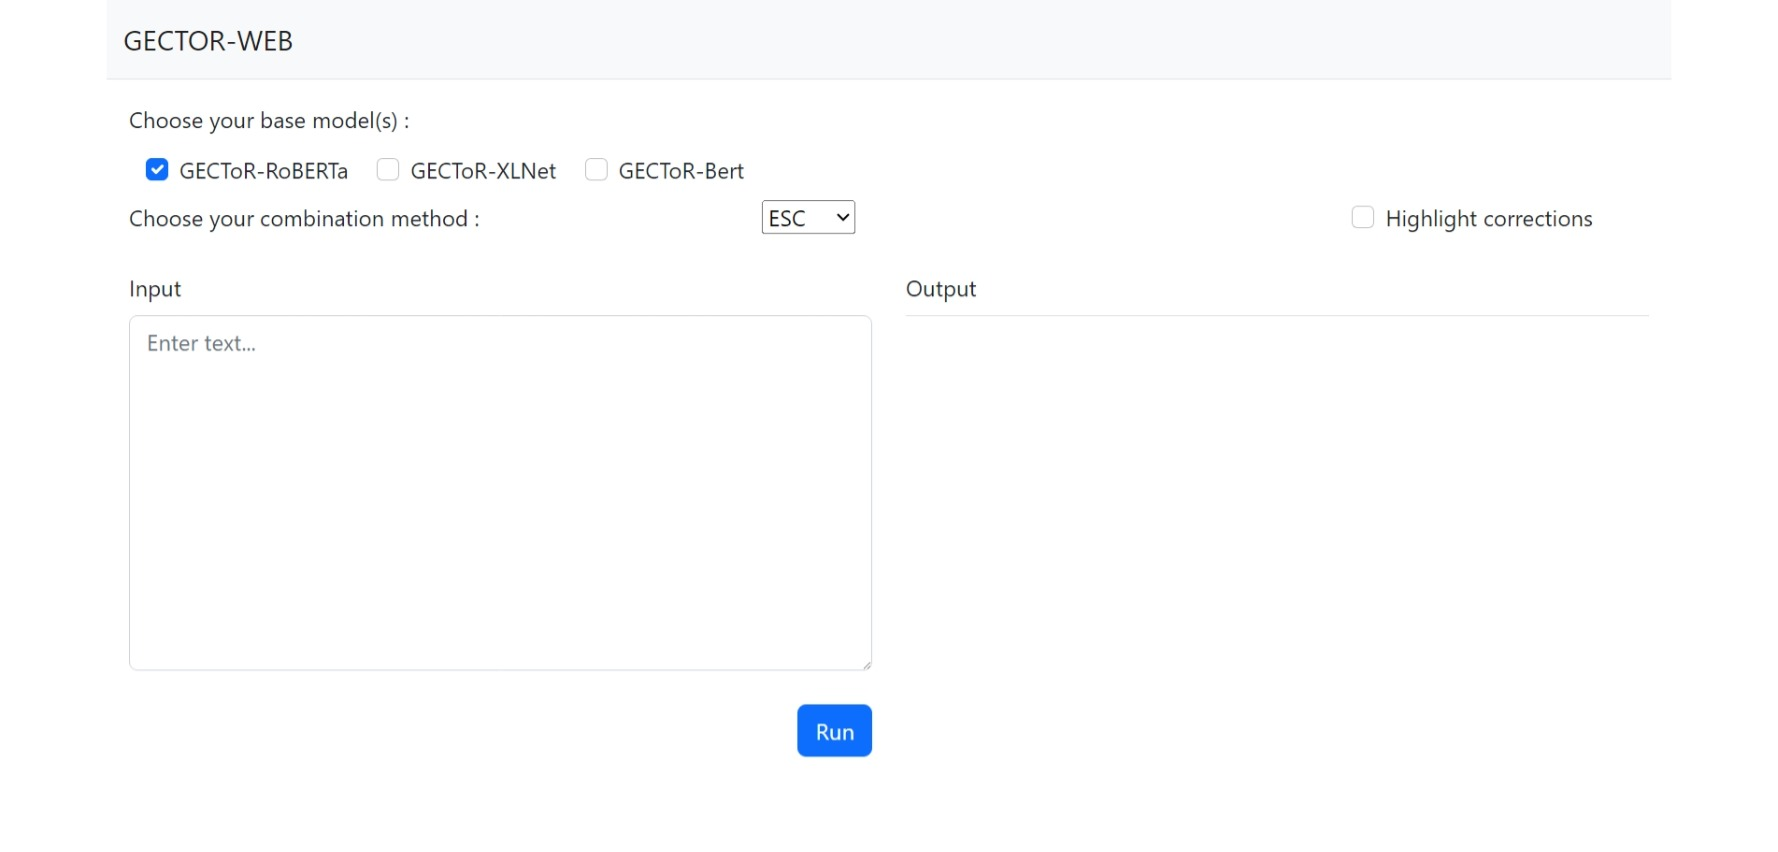
\includegraphics[width=\textwidth]{home}
  \end{center}
  \caption{The User Interface of GecWeb.}\label{fig:home}
\end{figure}

Figure \ref{fig:home} shows the user interface of GecWeb, it is consist of five main components: the input text area, the output text area, the model selection, the combination method, and the output mode.

\subsection{Layer design}

\subsection{Database design}

\section{Application Building}

\subsection{Libraries and Tools}

\subsection{Achievement}

\subsection{Illustration of main functions}

\section{Testing}

\section{Deployment}
